\documentclass[10pt]{article}
\usepackage{tikz}
\usetikzlibrary{shapes.misc}
\usepackage[margin=0cm]{geometry}
\pagestyle{empty}
\tikzstyle{every node}=[cross out, draw, red]

\begin{document}

\vspace*{\fill}
\begin{center}
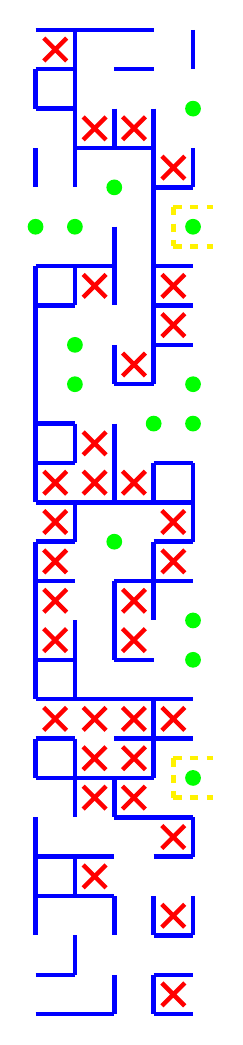
\begin{tikzpicture}[x=0.5cm, y=-0.5cm, ultra thick, blue]
% Walls
    \draw (0,0) -- (3,0);
    \draw (0,1) -- (1,1);
    \draw (2,1) -- (3,1);
    \draw (0,2) -- (1,2);
    \draw (1,3) -- (3,3);
    \draw (3,4) -- (4,4);
    \draw (0,6) -- (2,6);
    \draw (3,6) -- (4,6);
    \draw (0,7) -- (1,7);
    \draw (3,7) -- (4,7);
    \draw (3,8) -- (4,8);
    \draw (2,9) -- (3,9);
    \draw (0,10) -- (1,10);
    \draw (0,11) -- (1,11);
    \draw (3,11) -- (4,11);
    \draw (0,12) -- (4,12);
    \draw (0,13) -- (1,13);
    \draw (3,13) -- (4,13);
    \draw (0,14) -- (1,14);
    \draw (2,14) -- (4,14);
    \draw (0,16) -- (1,16);
    \draw (2,16) -- (3,16);
    \draw (0,17) -- (4,17);
    \draw (0,18) -- (1,18);
    \draw (2,18) -- (4,18);
    \draw (0,19) -- (3,19);
    \draw (2,20) -- (4,20);
    \draw (0,21) -- (2,21);
    \draw (3,21) -- (4,21);
    \draw (0,22) -- (2,22);
    \draw (3,23) -- (4,23);
    \draw (0,24) -- (1,24);
    \draw (3,24) -- (4,24);
    \draw (0,25) -- (2,25);
    \draw (3,25) -- (4,25);
    \draw (0,1) -- (0,2);
    \draw (0,3) -- (0,4);
    \draw (0,6) -- (0,12);
    \draw (0,13) -- (0,17);
    \draw (0,18) -- (0,19);
    \draw (0,20) -- (0,23);
    \draw (1,0) -- (1,4);
    \draw (1,6) -- (1,7);
    \draw (1,10) -- (1,11);
    \draw (1,12) -- (1,13);
    \draw (1,15) -- (1,17);
    \draw (1,18) -- (1,20);
    \draw (1,21) -- (1,22);
    \draw (1,23) -- (1,24);
    \draw (2,2) -- (2,3);
    \draw (2,5) -- (2,7);
    \draw (2,8) -- (2,9);
    \draw (2,10) -- (2,12);
    \draw (2,14) -- (2,16);
    \draw (2,19) -- (2,20);
    \draw (2,22) -- (2,23);
    \draw (2,24) -- (2,25);
    \draw (3,2) -- (3,9);
    \draw (3,11) -- (3,12);
    \draw (3,13) -- (3,15);
    \draw (3,17) -- (3,19);
    \draw (3,22) -- (3,23);
    \draw (3,24) -- (3,25);
    \draw (4,0) -- (4,1);
    \draw (4,3) -- (4,4);
    \draw (4,11) -- (4,13);
    \draw (4,20) -- (4,21);
    \draw (4,22) -- (4,23);
% Pillars
    \fill[green] (4,2) circle(0.2);
    \fill[green] (2,4) circle(0.2);
    \fill[green] (0,5) circle(0.2);
    \fill[green] (1,5) circle(0.2);
    \fill[green] (4,5) circle(0.2);
    \fill[green] (1,8) circle(0.2);
    \fill[green] (1,9) circle(0.2);
    \fill[green] (4,9) circle(0.2);
    \fill[green] (3,10) circle(0.2);
    \fill[green] (4,10) circle(0.2);
    \fill[green] (2,13) circle(0.2);
    \fill[green] (4,15) circle(0.2);
    \fill[green] (4,16) circle(0.2);
    \fill[green] (4,19) circle(0.2);
% Inner points in accessible cul-de-sacs
    \node at (0.5,0.5) {};
    \node at (1.5,2.5) {};
    \node at (2.5,2.5) {};
    \node at (3.5,3.5) {};
    \node at (1.5,6.5) {};
    \node at (3.5,6.5) {};
    \node at (3.5,7.5) {};
    \node at (2.5,8.5) {};
    \node at (1.5,10.5) {};
    \node at (0.5,11.5) {};
    \node at (1.5,11.5) {};
    \node at (2.5,11.5) {};
    \node at (0.5,12.5) {};
    \node at (3.5,12.5) {};
    \node at (0.5,13.5) {};
    \node at (3.5,13.5) {};
    \node at (0.5,14.5) {};
    \node at (2.5,14.5) {};
    \node at (0.5,15.5) {};
    \node at (2.5,15.5) {};
    \node at (0.5,17.5) {};
    \node at (1.5,17.5) {};
    \node at (2.5,17.5) {};
    \node at (3.5,17.5) {};
    \node at (1.5,18.5) {};
    \node at (2.5,18.5) {};
    \node at (1.5,19.5) {};
    \node at (2.5,19.5) {};
    \node at (3.5,20.5) {};
    \node at (1.5,21.5) {};
    \node at (3.5,22.5) {};
    \node at (3.5,24.5) {};
% Entry-exit paths without intersections
    \draw[dashed, yellow] (3.5,4.5) -- (4.5,4.5);
    \draw[dashed, yellow] (3.5,5.5) -- (4.5,5.5);
    \draw[dashed, yellow] (3.5,18.5) -- (4.5,18.5);
    \draw[dashed, yellow] (3.5,19.5) -- (4.5,19.5);
    \draw[dashed, yellow] (3.5,4.5) -- (3.5,5.5);
    \draw[dashed, yellow] (3.5,18.5) -- (3.5,19.5);
\end{tikzpicture}
\end{center}
\vspace*{\fill}

\end{document}
